\documentclass[11pt,fleqn]{article}
\usepackage{pgf,tikz}
\usepackage[ngerman]{babel}
\usepackage[utf8]{inputenc}
\usepackage[T1]{fontenc}
\usepackage{float}
\usepackage{mathtools}
\usepackage{fancyhdr}
\usepackage[margin=1.2in]{geometry}
\usepackage{graphicx}
\usepackage{lmodern}
\usepackage{circuitikz}
\usepackage{pgfplots}
\usepackage{pgfplotstable}
\usepackage{amsmath}
\usepackage{amssymb}
\usepackage{amsfonts}
\usepackage{siunitx}
\usepackage[backend=biber, citestyle=alphabetic, style=alphabetic]{biblatex}
\usepackage{pdfpages}


\bibliography{literatur.bib}

\parindent 0pt
\parskip 10pt
\newcommand{\degre}{\ensuremath{^\circ}}

\title{Technische Optik \\ Praktikum Linsenfehler}
\date{4. Juni 2015}
\author{Hans Herrmann \and Felix Kayser \and Hermann Pommerenke \and Tino Steinmetz}

\begin{document}
	\pagenumbering{gobble}
	\begin{figure}[t]
	    \centering
	    
\includegraphics[width=115mm]{img/UNI-Logo_Siegel_4c_115mm_07.png}
	\end{figure}

	\maketitle
	
	\thispagestyle{empty}

	\newpage
	\pagenumbering{Roman}
	\pagestyle{headings}
	\tableofcontents
	
	\everymath{\displaystyle} % Jede Formel im Displaystyle
	
	\newpage
	\pagenumbering{arabic}

	\section{Einleitung}
	
	\clearpage
	\section{Versuchsaufbau}

\begin{figure}[h!]
	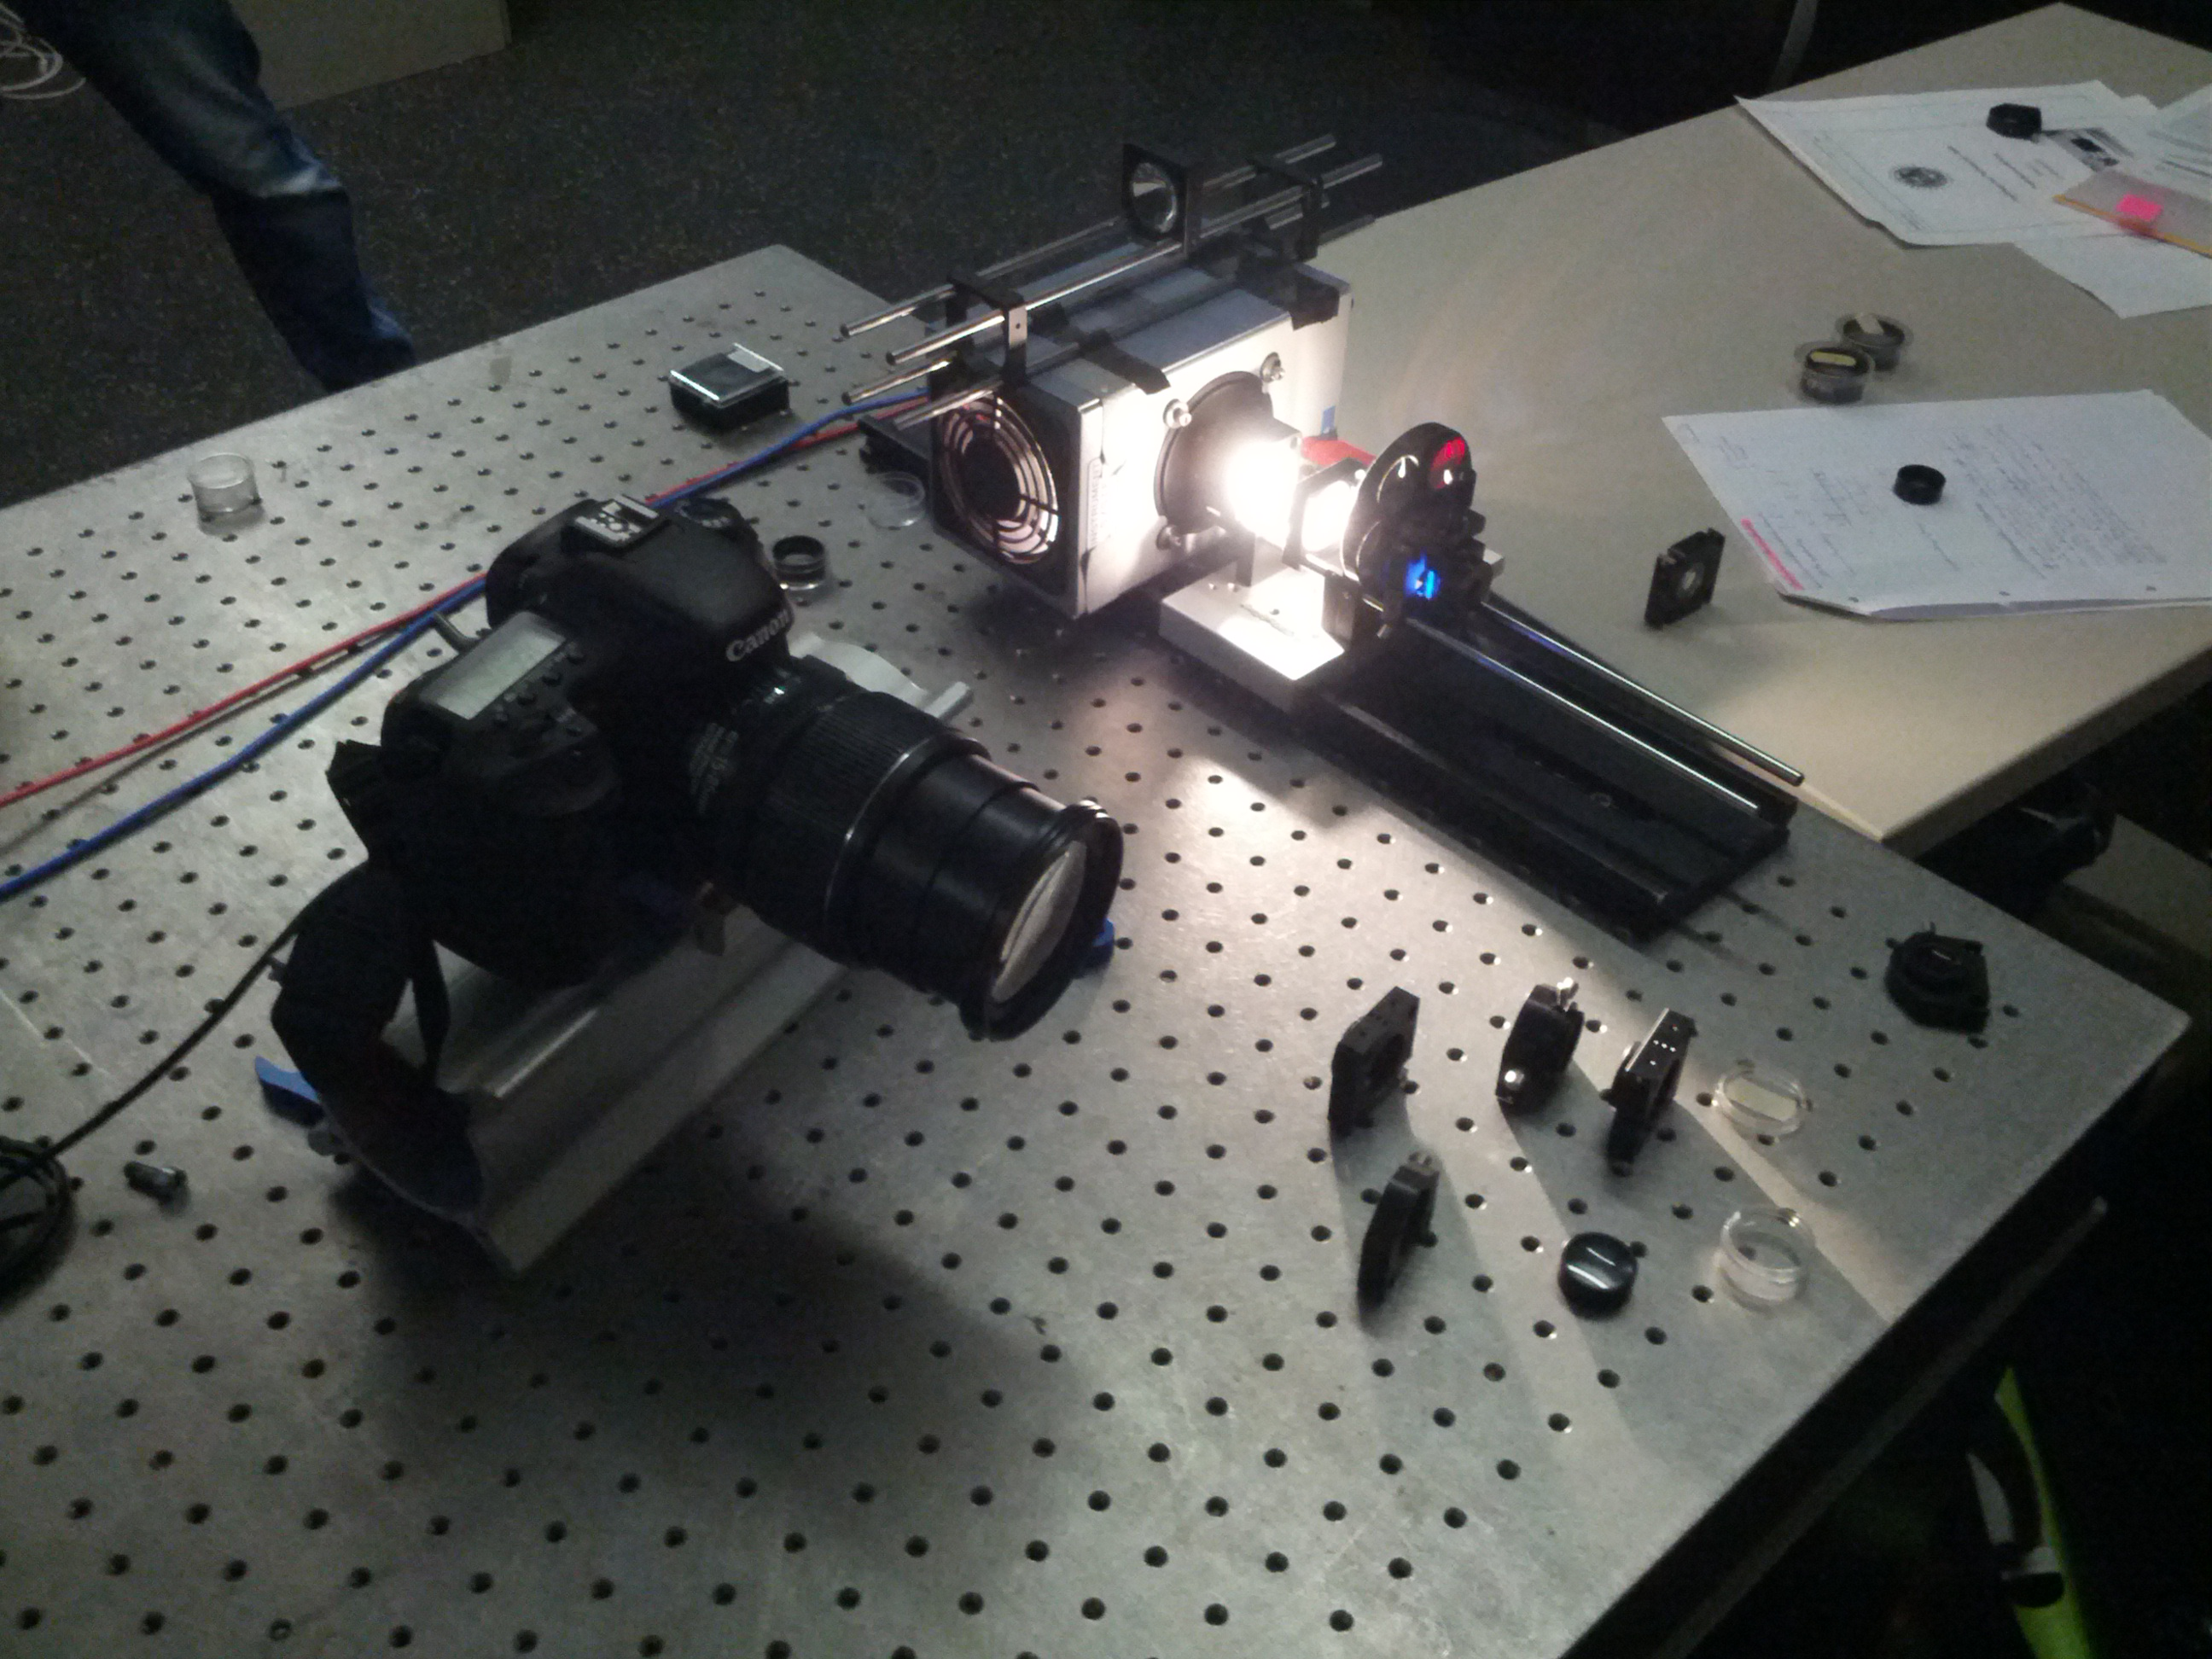
\includegraphics[width=\linewidth]{img/Versuchsaufbau}
	\caption{Der Versuchsaufbau}
	\label{fig:versuchsaufbau}
\end{figure}

Der Versuchsaufbau wurde mithilfe des Mikro-Bank-Systems Linos realisiert. Der lineare Aufbau bestand aus einer Lichtquelle (Weißlicht), einer Streuscheibe, einem Farbfilter, einem Objekt und einer zu untersuchenden Linse. \newline 
Das Licht der Quelle wurde zuerst in der Streuscheibe gebrochen, um diffuses Licht zu erhalten. Der darauffolgende Farbfilter war einstellbar: Es war sowohl möglich das Licht ungefiltert passieren zu lassen, als auch einen roten, blauen oder grünen Filter zu verwenden. Direkt hinter dem Filter war das Beobachtungsobjekt angebracht. Hierfür eigneten sich beispielsweise der Siemensstern, eine Skala oder ein Netzchen (feines Raster). Darauffolgend wurden Linsen auf das Mikro-Bank-System gesteckt. Diese Linsen haben jeweils einen zu untersuchenden Abbildungsfehler besonders deutlich gezeigt. Um diesen Fehler sichtbar zu machen, konnten die Linsen zur Fokussierung verschoben werden. 
Die Abbildung wurde auf einem weißen Papierschirm realisiert. Das hatte den Vorteil gegenüber eines CCD Sensors, dass das Bild mit dem Auge wahrgenommen werden konnte. Somit wurden das Auswählen der für den gewünschten Fehler geeignetsten Linse und das Fokussieren vereinfacht.
Nachdem eine für das Protokoll geeignete Abbildung auf dem Schirm realisiert werden konnte, wurde der Schirm mit einer Spiegelreflexkamera fotografiert. Hierbei war zu beachten, einen manuellen Fokus und Weißabgleich zu benutzen, welche vorher fest eingestellt werden mussten. 
	
	\clearpage
	\section{Auswertung}

\subsection{Sphärische Aberration}

\subsection{Koma}

\begin{figure}[htb]
	\begin{minipage}[t]{0.32\textwidth}
		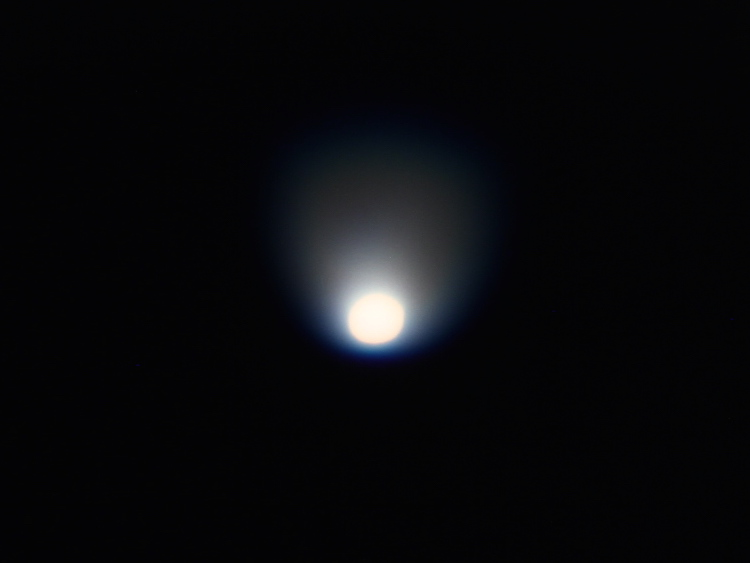
\includegraphics[width=\linewidth]{img/Koma/Prakt_Linsenfehler_2015_06_04_097}
		\label{fig:koma_stark}
		\caption{Starkes Koma am Außenrand der Linse}
	\end{minipage}
	\hfill
	\begin{minipage}[t]{0.32\textwidth}
		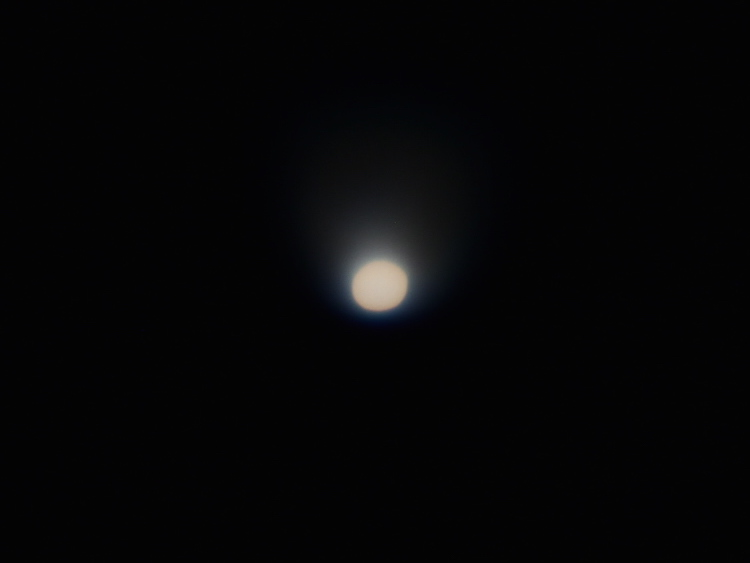
\includegraphics[width=\linewidth]{img/Koma/Prakt_Linsenfehler_2015_06_04_096}
		\label{fig:koma_schwach}
		\caption{Schwaches Koma nahe der optischen Achse}
	\end{minipage}
	\hfill
	\begin{minipage}[t]{0.32\textwidth}
		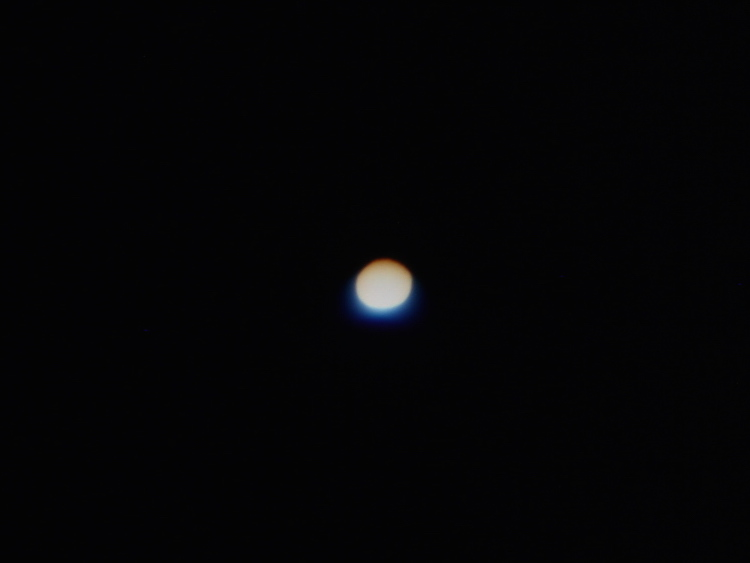
\includegraphics[width=\linewidth]{img/Koma/Prakt_Linsenfehler_2015_06_04_099}
		\label{fig:koma_korrigiert}
		\caption{Abbildung mit Korrektur der Koma}
	\end{minipage}	
\end{figure}

\subsection{Astigmatismus}

\begin{figure}[htb]
	\begin{minipage}[t]{0.48\textwidth}
		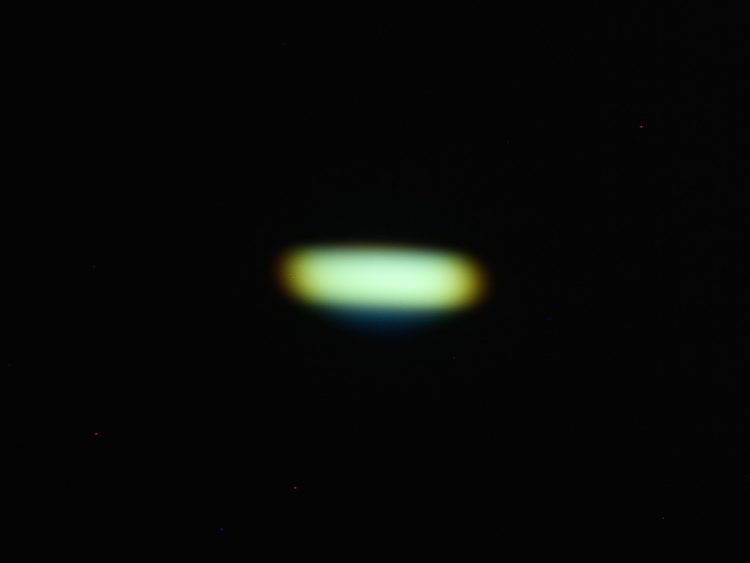
\includegraphics[width=\linewidth]{img/Astigmatismus/Prakt_Linsenfehler_2015_06_04_087_saggital}
		\label{fig:astigmatismus_saggital}
		\caption{Abbildung der Saggitalebene}
	\end{minipage}
	\hfill
	\begin{minipage}[t]{0.48\textwidth}
		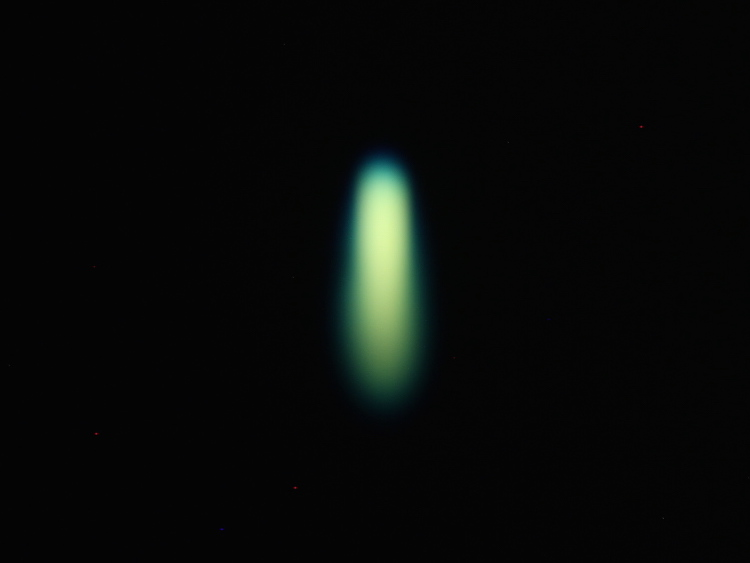
\includegraphics[width=\linewidth]{img/Astigmatismus/Prakt_Linsenfehler_2015_06_04_088_meridional}
		\label{fig:astigmatismus_meridional}
		\caption{Abbildung der Meridionalebene}
	\end{minipage}
	
	\vspace{0.5cm}
	
	\begin{minipage}[t]{0.48\textwidth}
		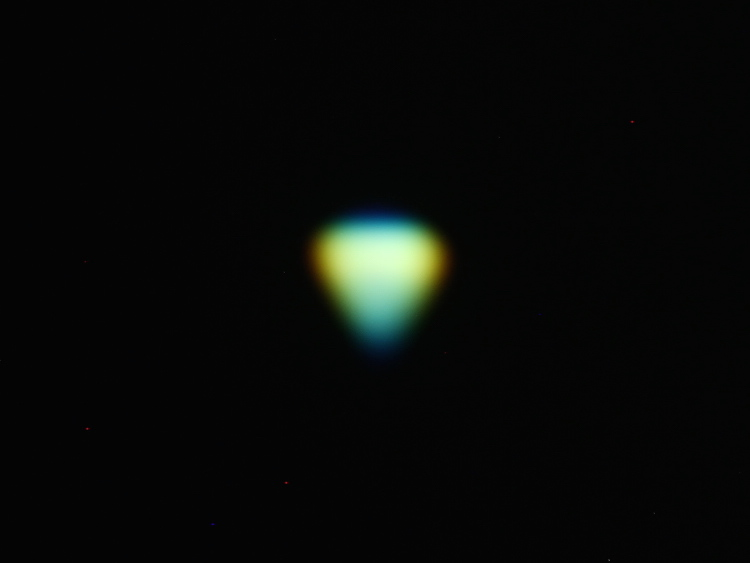
\includegraphics[width=\linewidth]{img/Astigmatismus/Prakt_Linsenfehler_2015_06_04_089_mittenfokus}
		\label{fig:astigmatismus_mittenfokus}
		\caption{Fokus zwischen meridionaler und saggitaler Abbildung}
	\end{minipage}
	\hfill
	\begin{minipage}[t]{0.48\textwidth}
		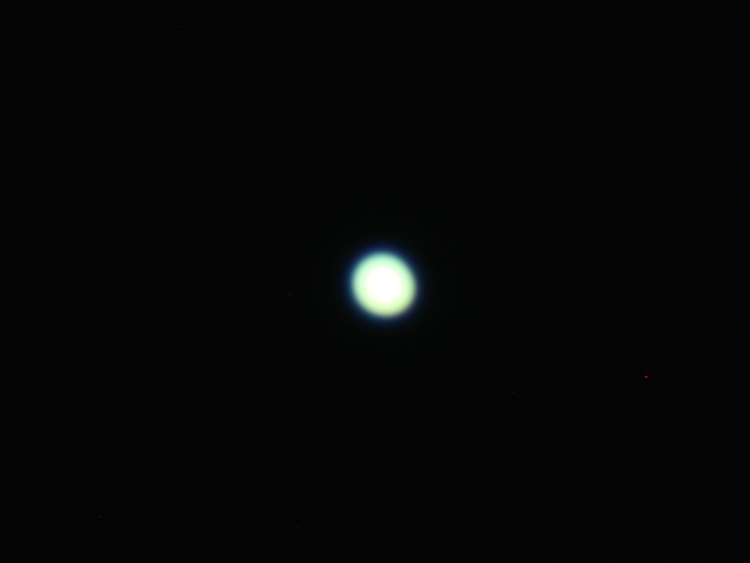
\includegraphics[width=\linewidth]{img/Astigmatismus/Prakt_Linsenfehler_2015_06_04_086}
		\label{fig:astigmatismus_korrigiert}
		\caption{Korrektur des Astigmatismus}
	\end{minipage}
\end{figure}

\subsection{Bildfeldwölbung}

\begin{figure}[htb]
	\begin{minipage}[t]{0.48\textwidth}
		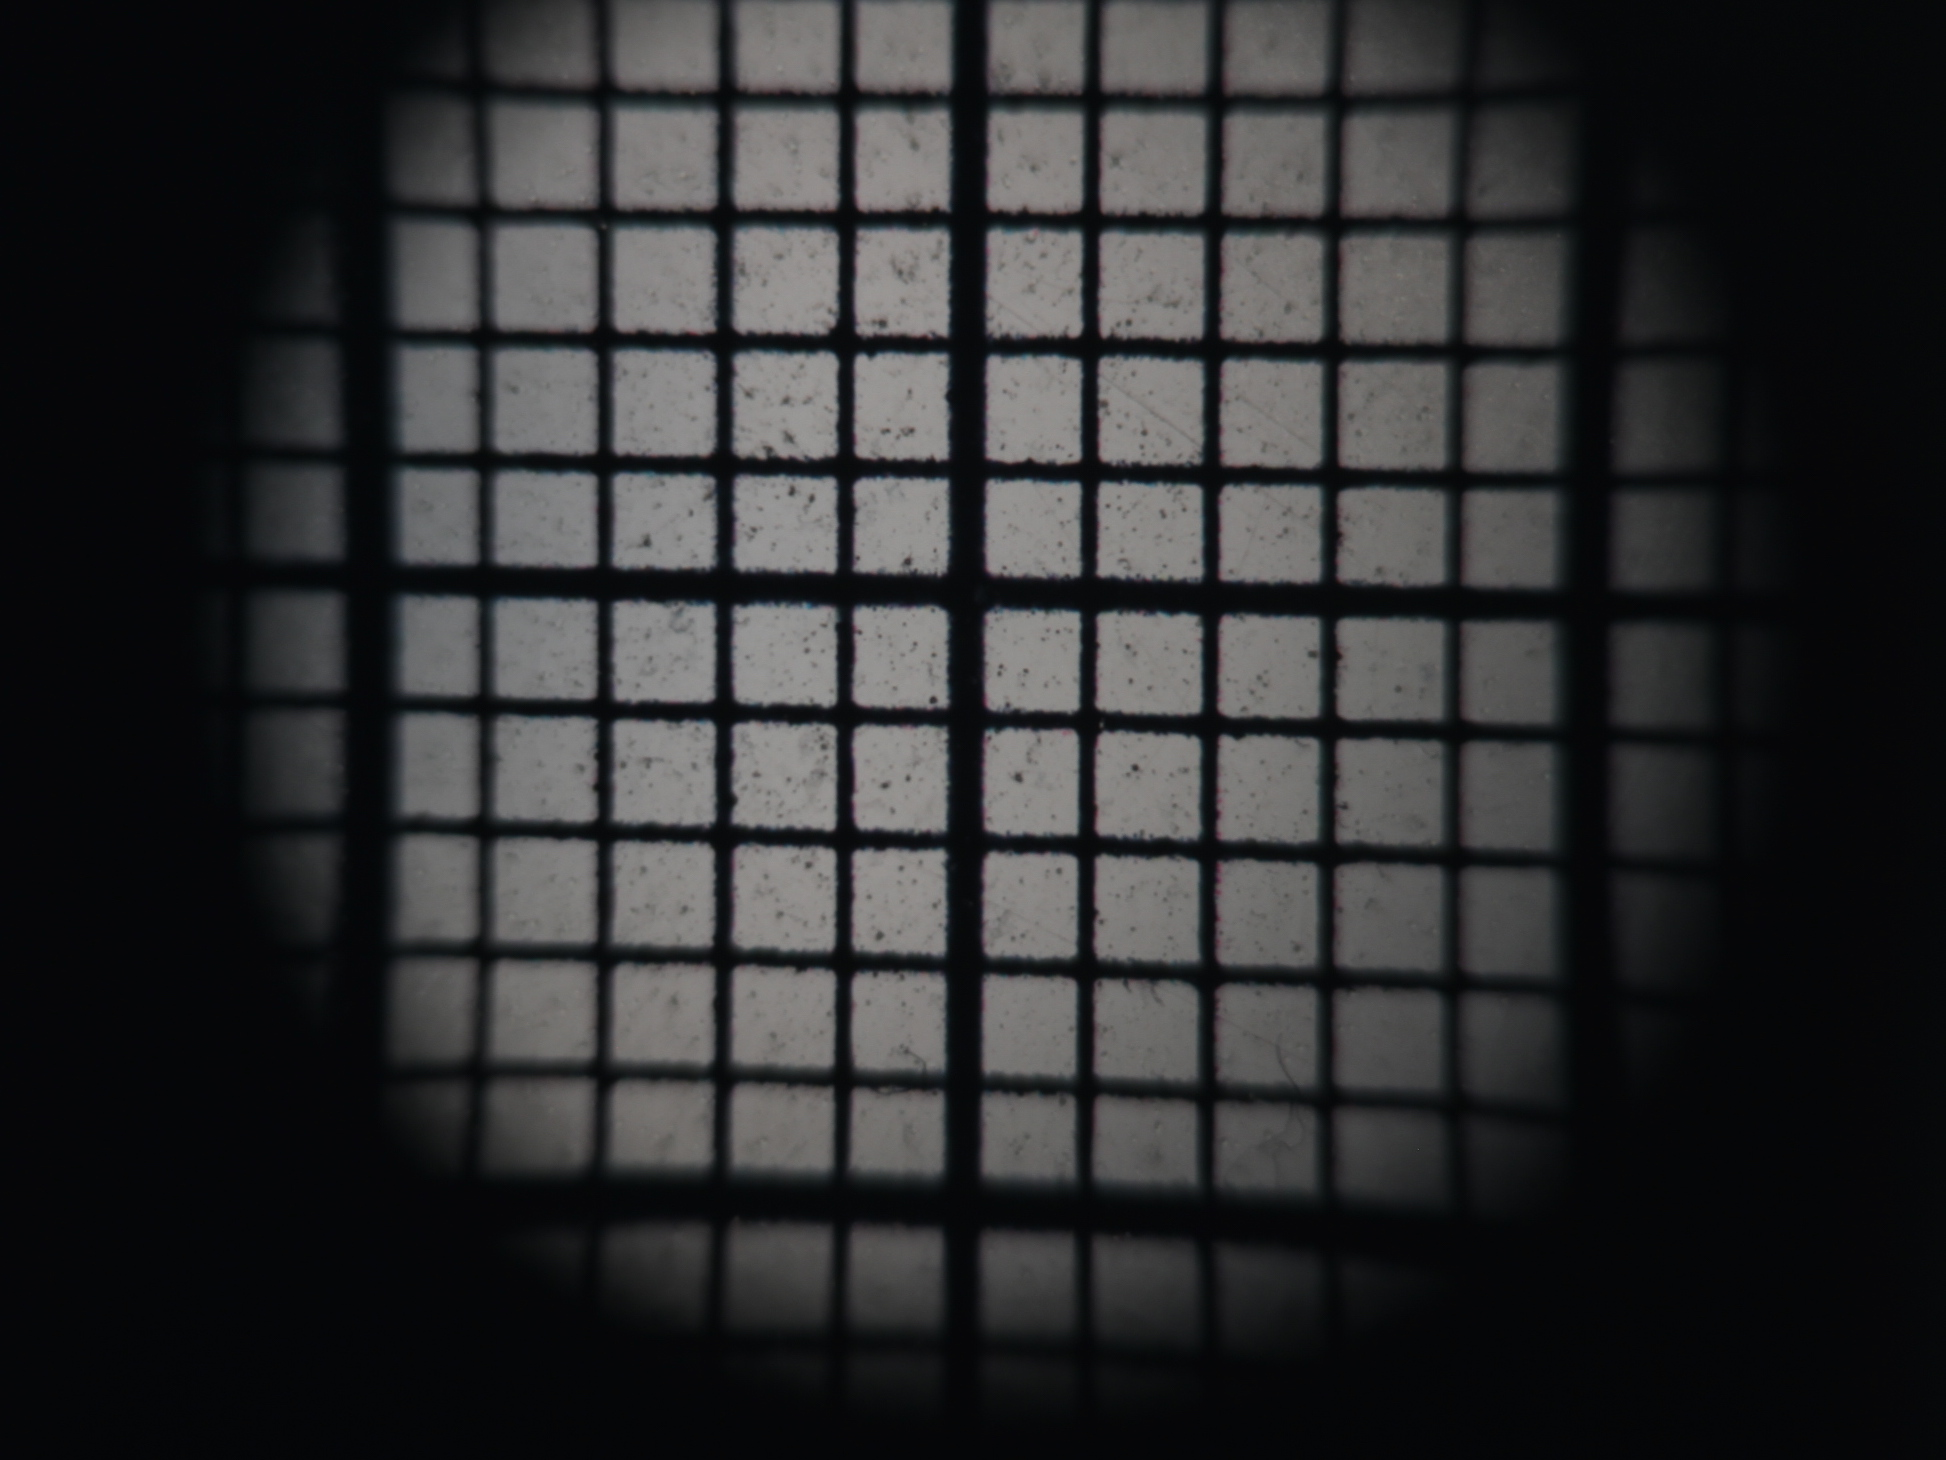
\includegraphics[width=\linewidth]{img/Bildwoelbung/Prakt_Linsenfehler_2015_06_04_074}
		\label{fig:bildwoelbung_aussen}
		\caption{Unschärfe am Außenrand des Gitters}
	\end{minipage}
	\hfill
	\begin{minipage}[t]{0.48\textwidth}
		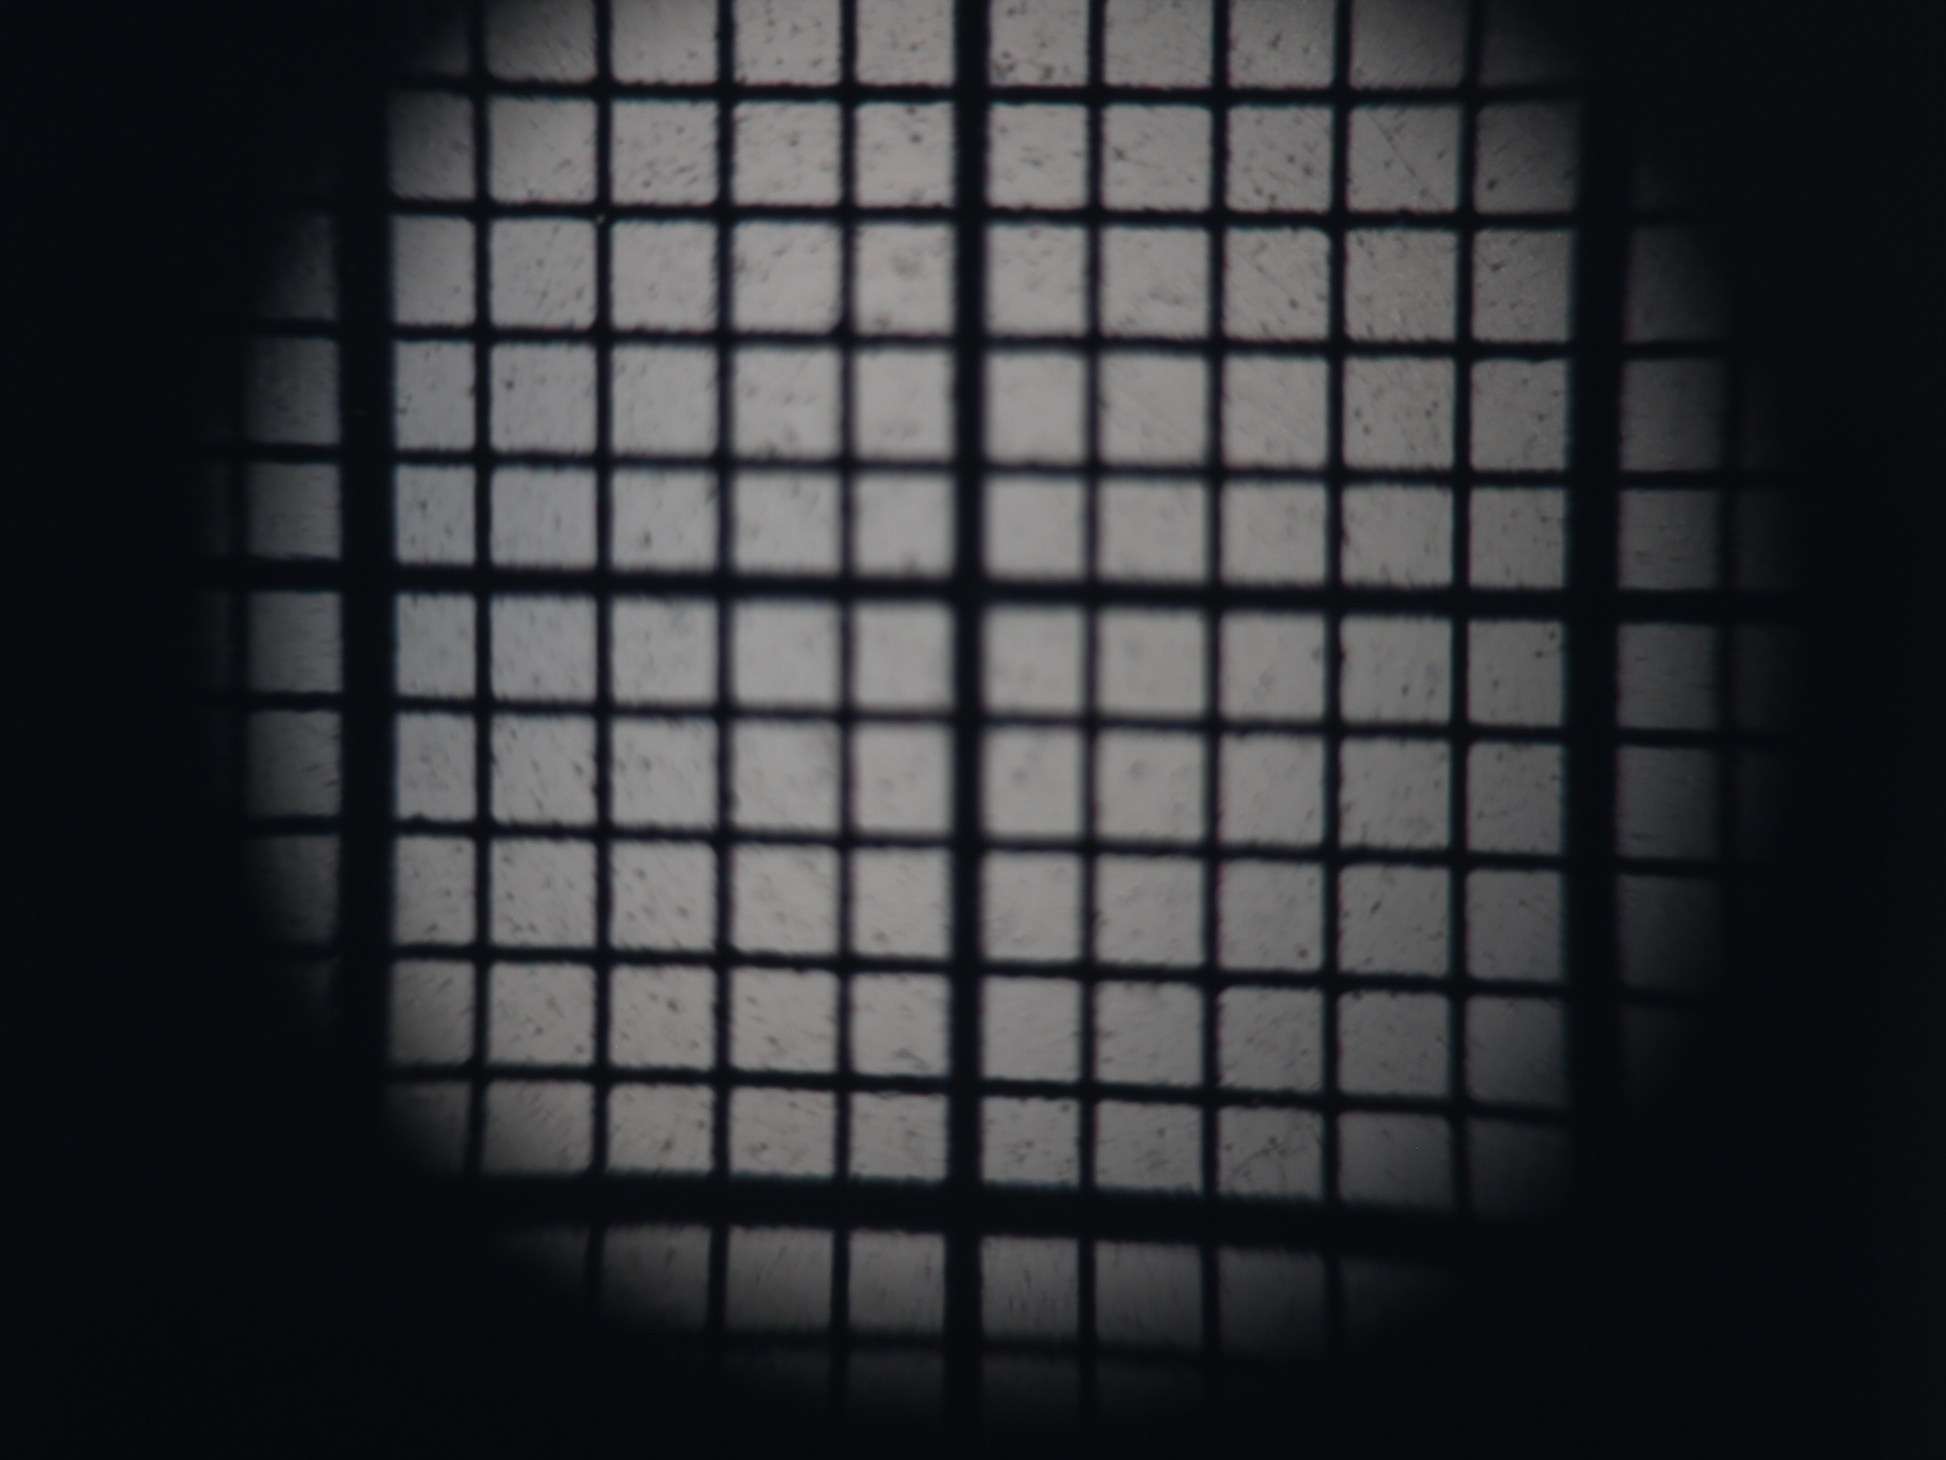
\includegraphics[width=\linewidth]{img/Bildwoelbung/Prakt_Linsenfehler_2015_06_04_075}
		\label{fig:bildwoelbung_korrigiert}
		\caption{Unschärfe in der Mitte des Gitters}
	\end{minipage}
\end{figure}

\begin{figure}[htb]
	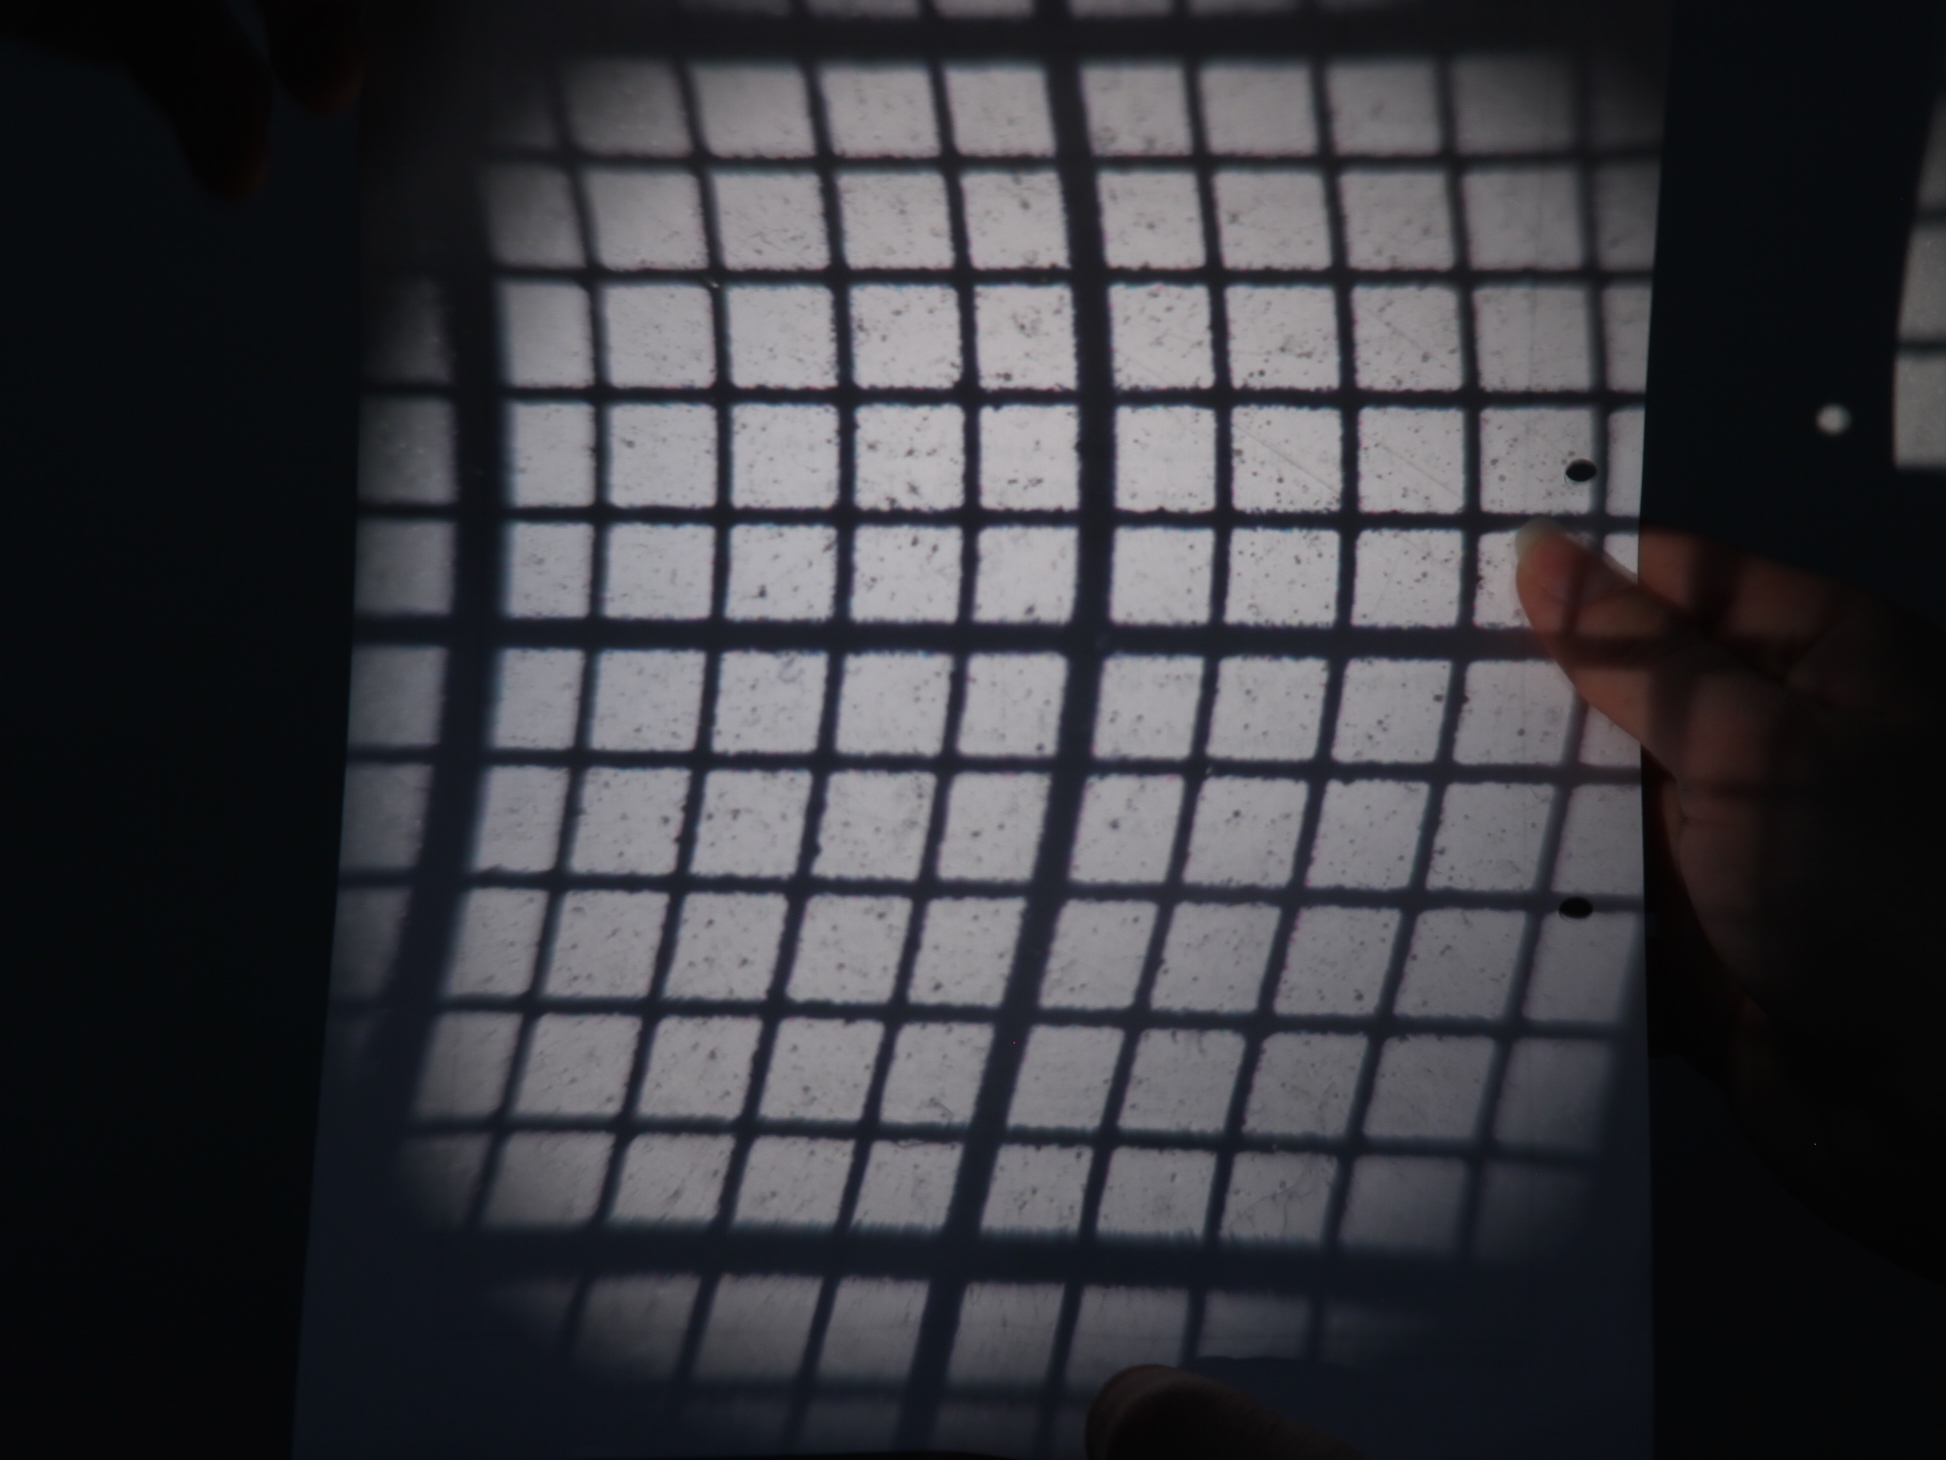
\includegraphics[width=\linewidth]{img/Bildwoelbung/Prakt_Linsenfehler_2015_06_04_076}
	\label{fig:bildwoelbung_korrigiert}
	\caption{Korrektur der Bildfeldwölbung durch gekrümmten Projektionsschirm}
\end{figure}

\subsection{Verzeichnung}

\begin{figure}[htb]
	\begin{minipage}[t]{0.48\textwidth}
		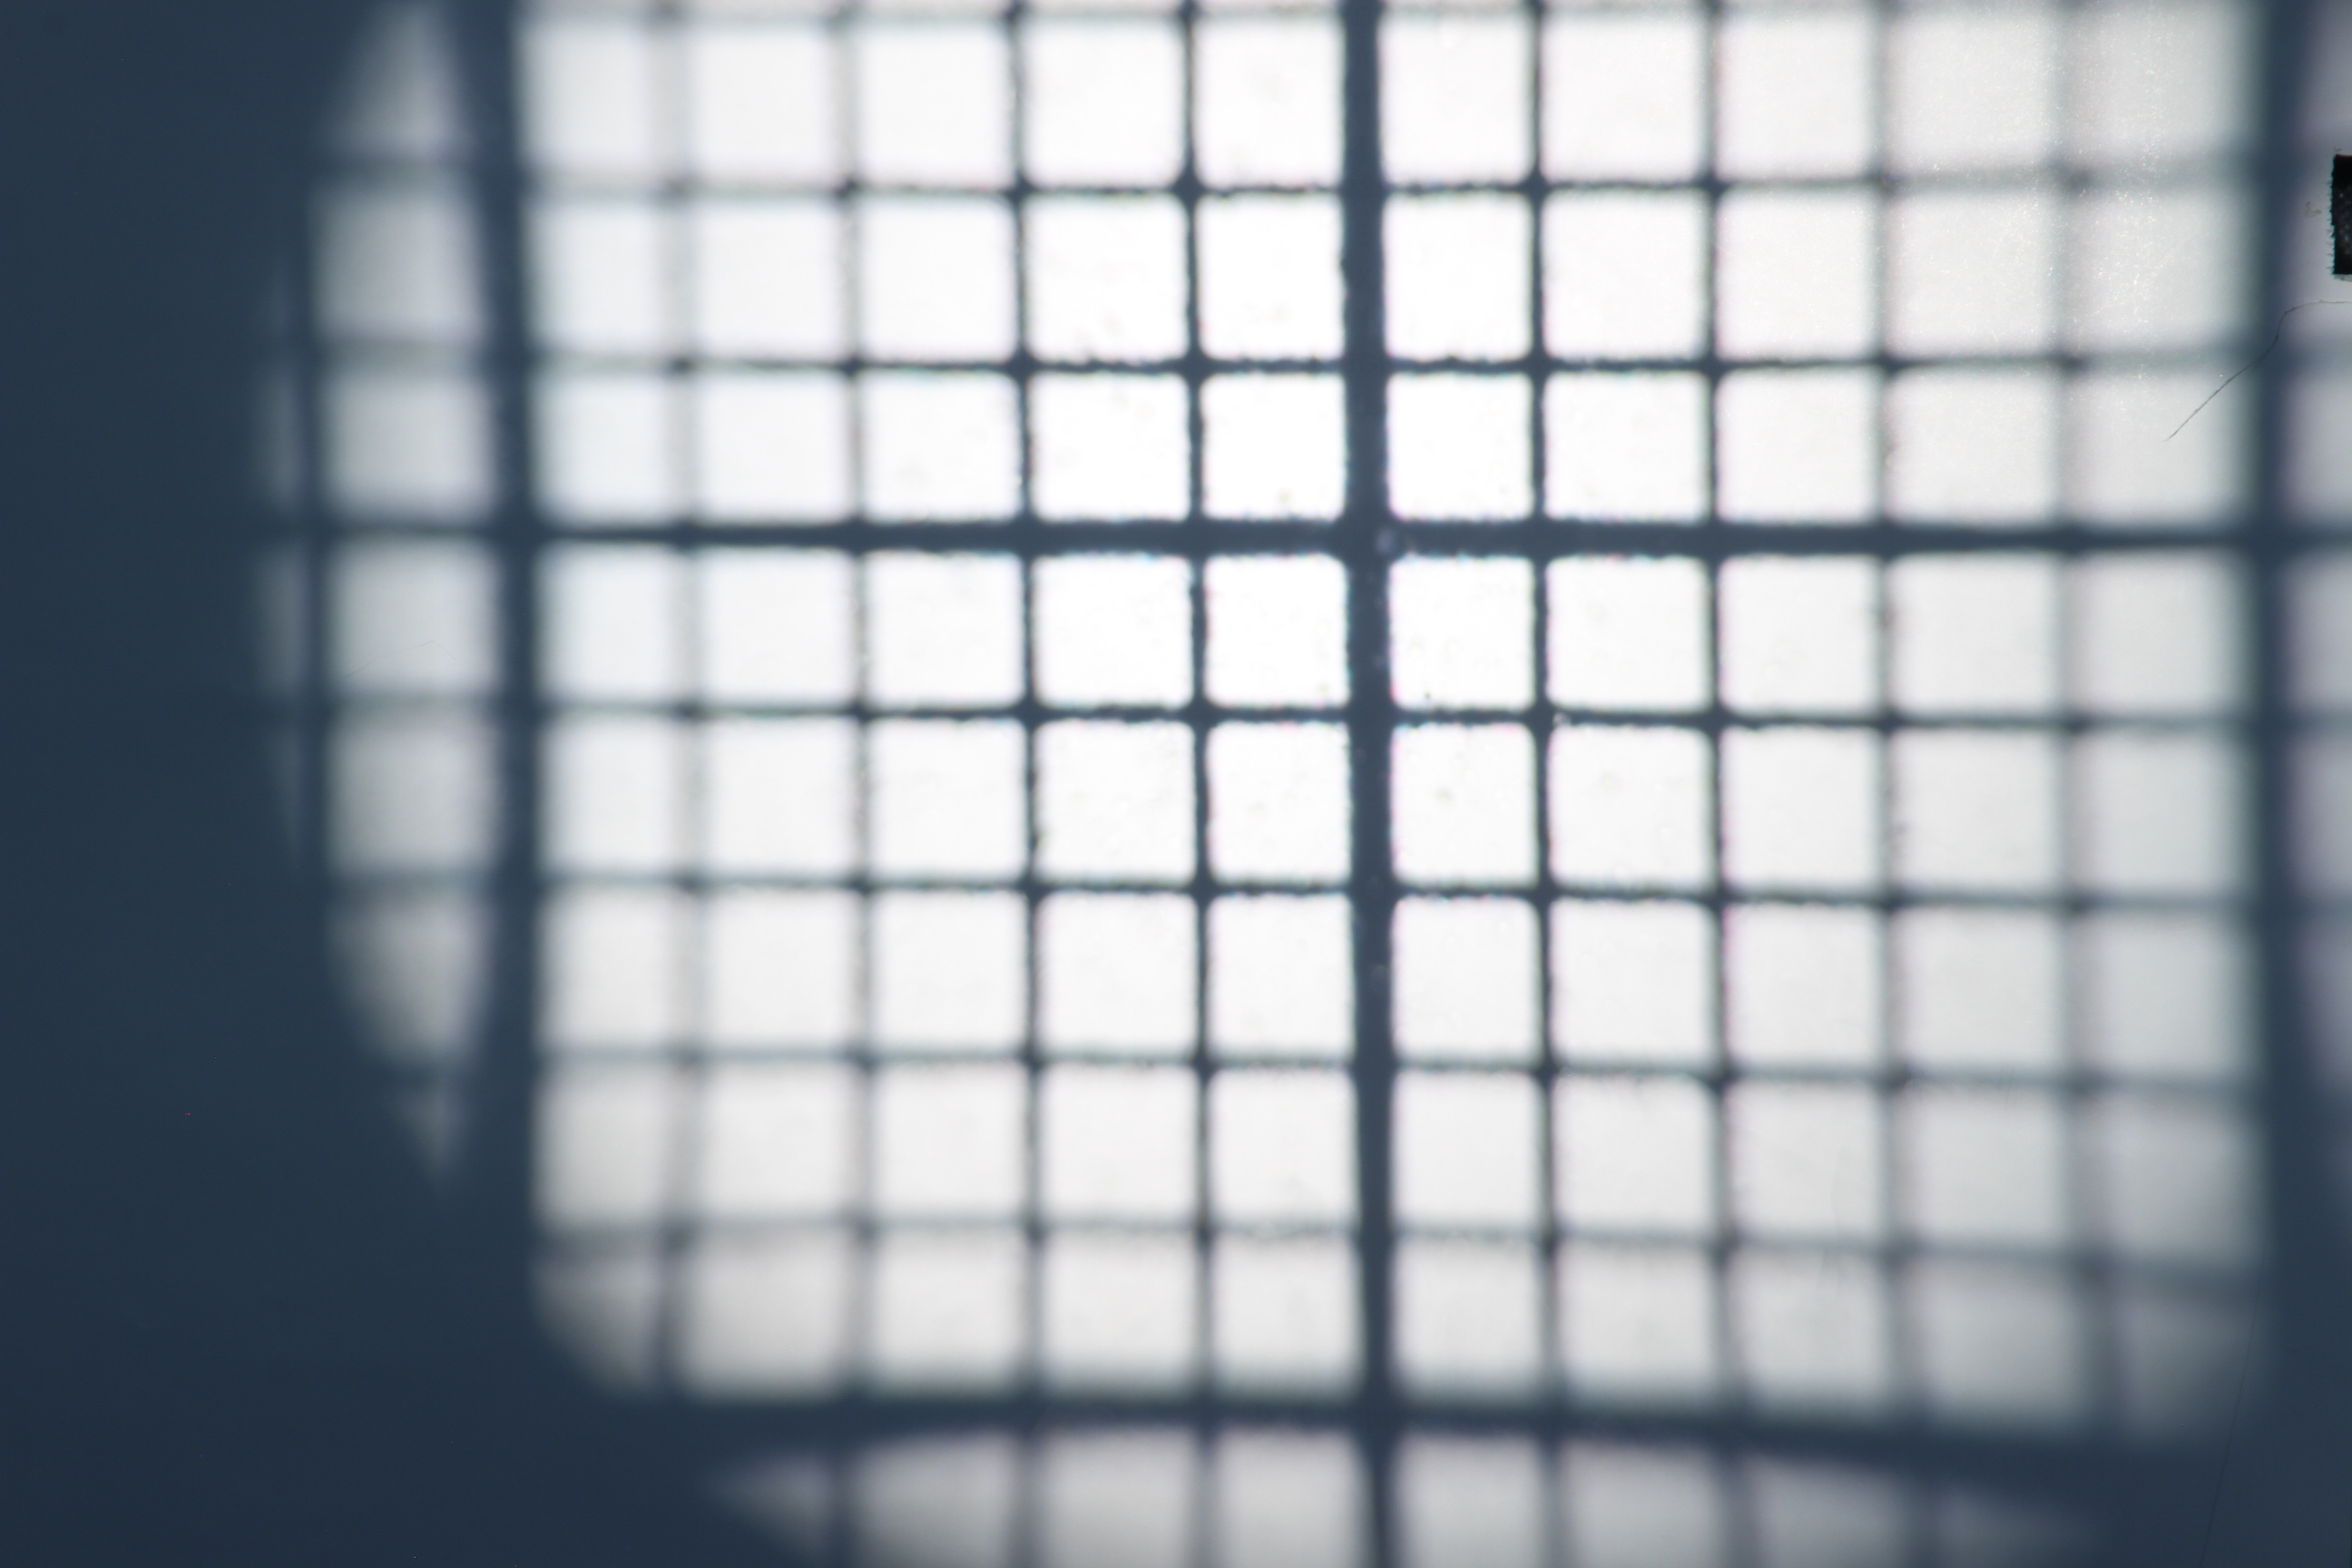
\includegraphics[width=\linewidth]{img/Verzeichnung/Prakt_Linsenfehler_2015_06_04_082}
		\label{fig:verzeichnung}
		\caption{Am Rand des Gitters erkennbare Krümmung}
	\end{minipage}
	\hfill
	\begin{minipage}[t]{0.48\textwidth}
		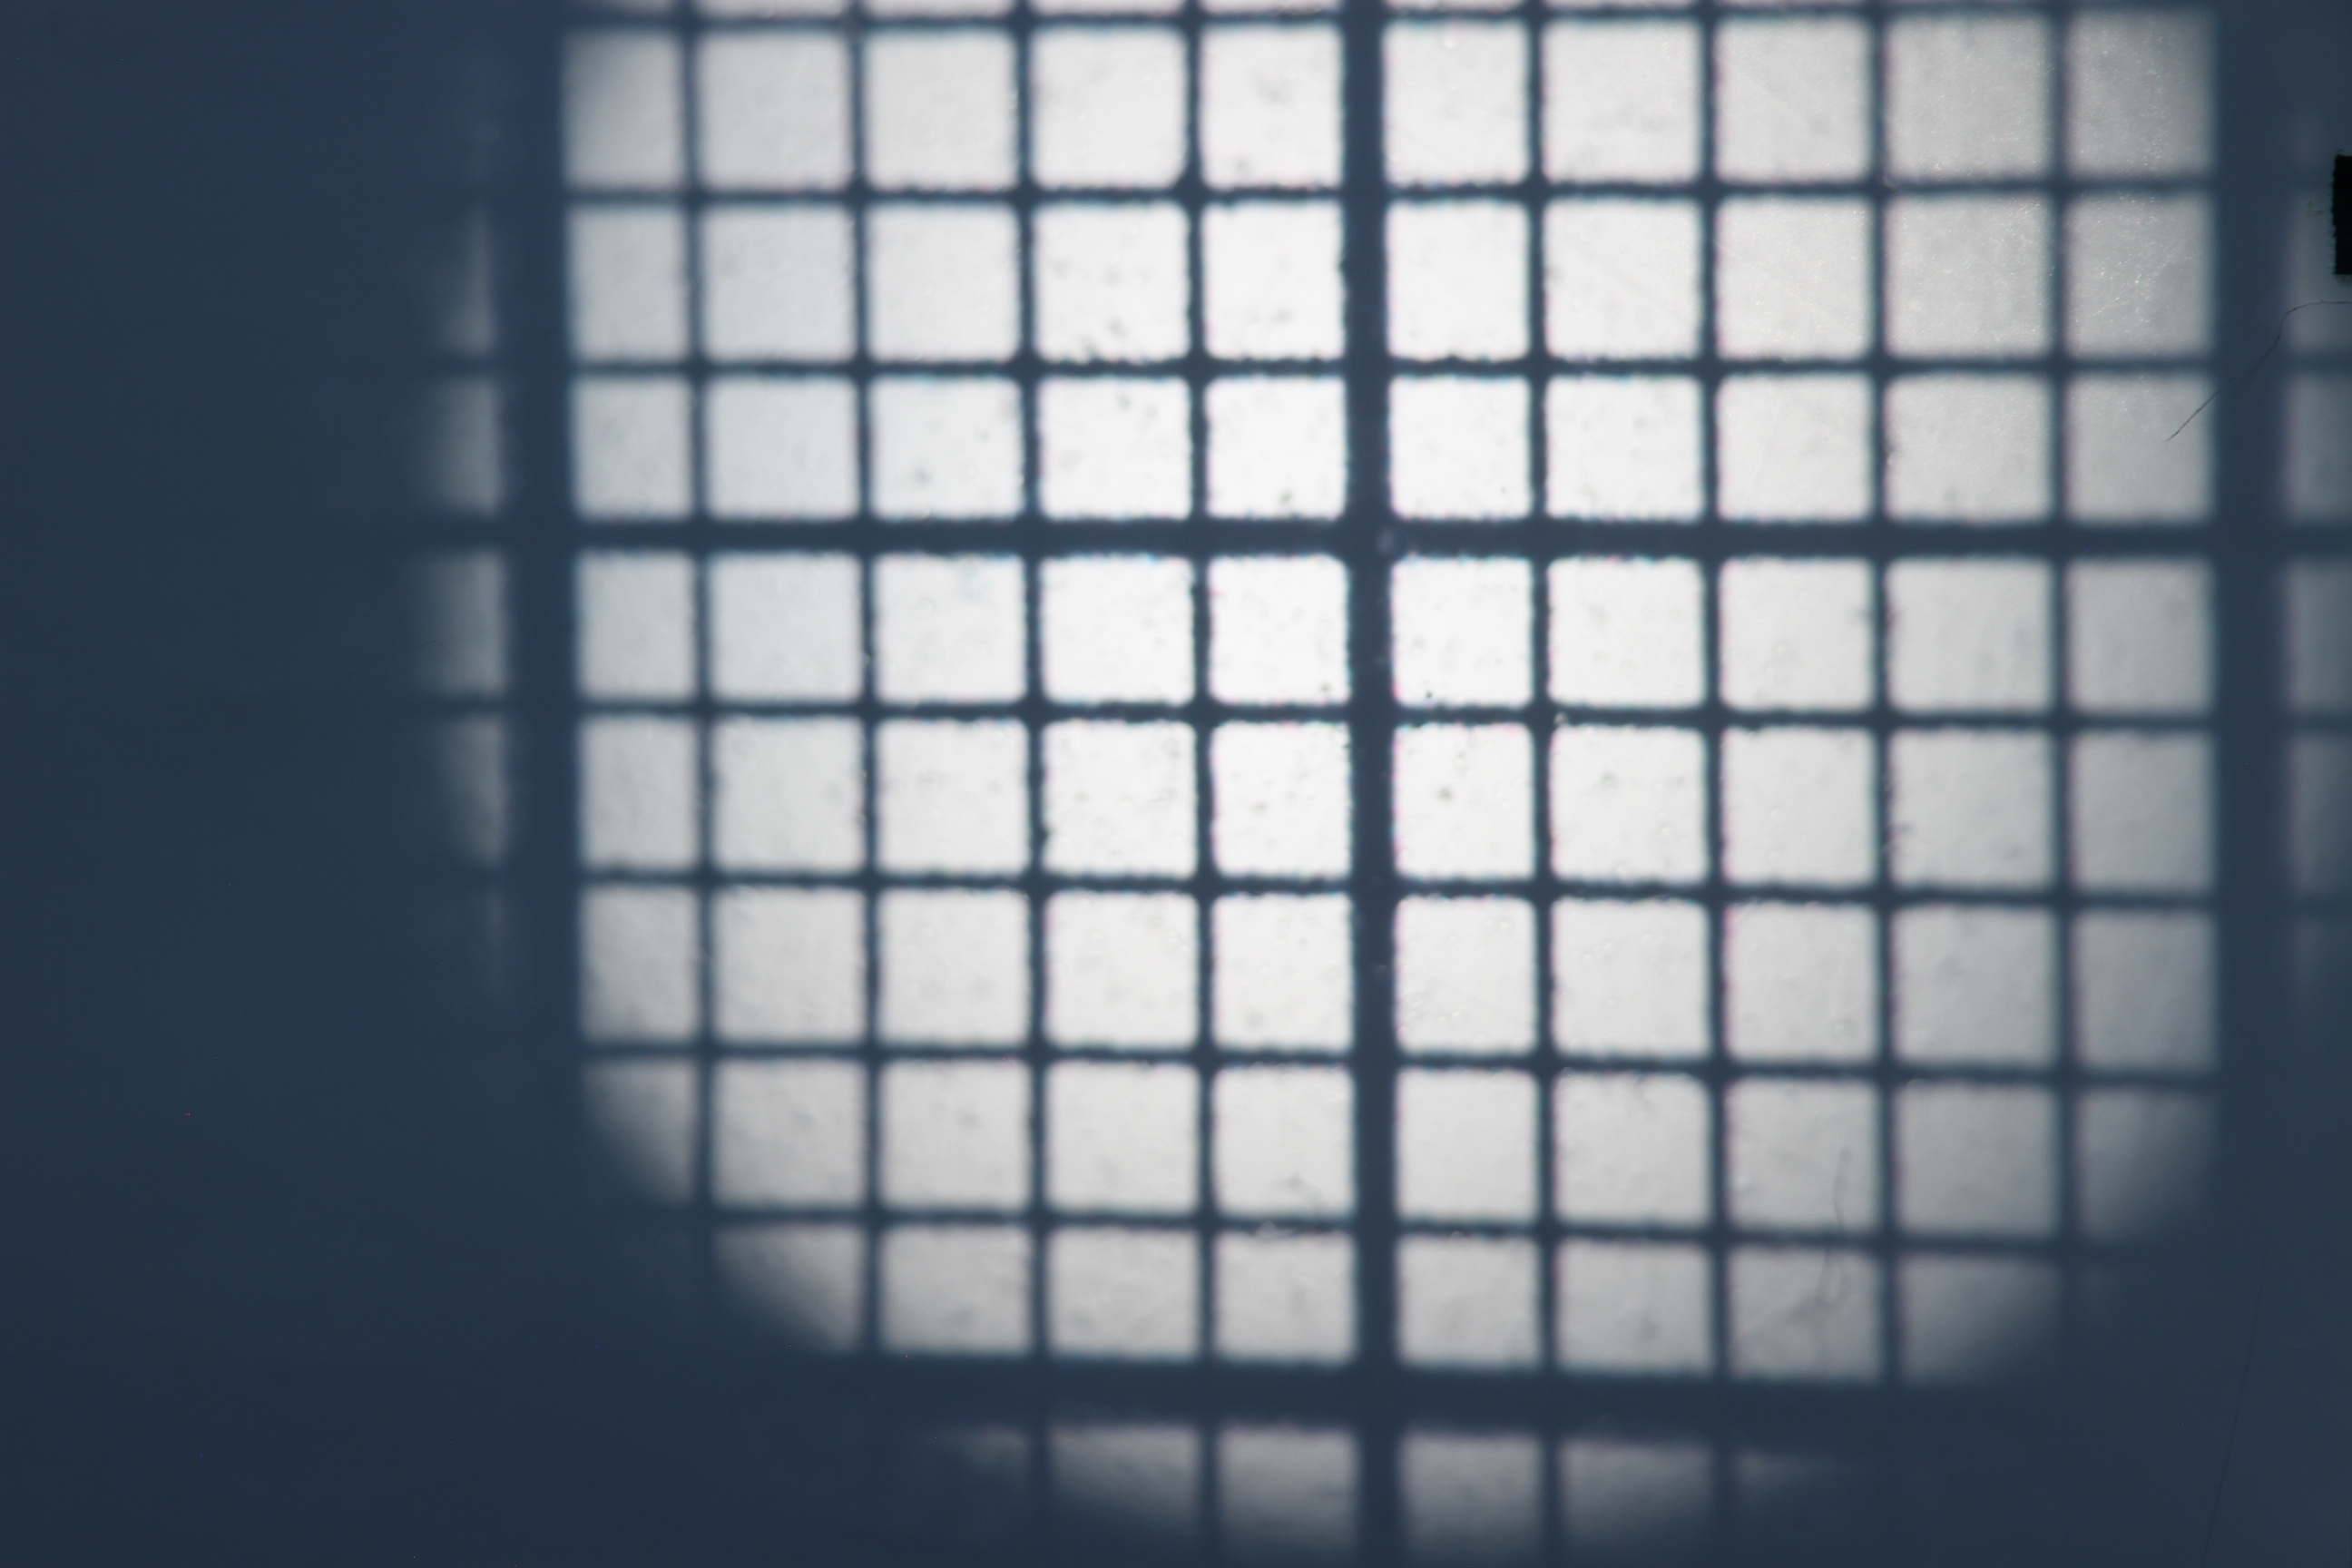
\includegraphics[width=\linewidth]{img/Verzeichnung/Prakt_Linsenfehler_2015_06_04_083}
		\label{fig:verzeichnung_korrigiert}
		\caption{Korrektur der Verzeichnung}
	\end{minipage}
\end{figure}

\subsection{chromatische Aberration}
	
	\clearpage
	\section{Anhang}


	
	\clearpage
	\printbibliography
\end{document}
